\documentclass[a4paper]{article}
    \usepackage[T1]{fontenc}    %Codifica dei font
    \usepackage[utf8]{inputenc} %Lettere accentate da tastiera
    \usepackage[english]{babel} %Lingua del documento
    \usepackage{tabularx}       % extra features for tabular environment
    \usepackage{booktabs}
    \usepackage[table,xcdraw]{xcolor}
    \usepackage{siunitx}
    \usepackage{fancyvrb}
    \sisetup{output-decimal-marker={,}}
    \usepackage{graphicx} % takes care of graphic including machinery
    \usepackage[margin=0.75in,a4paper]{geometry} % decreases margins
    \usepackage[final]{hyperref} % adds hyper links inside the generated pdf file
    % \usepackage{minted}

    \newcommand{\polito }{\emph{Politecnico di Torino}}
    \newcommand{\oses}{\emph{Energy Management for IoT}}


    \begin{document}
    \title{
        Energy Management for IoT - Report Lab 01 \\[0.5cm]
        
\includegraphics[width=0.15\textwidth]{PoliLogo.png}%
    }
    \author{Samuele Yves Cerini (s256813)}
    \date{\today}
    \maketitle

    \tableofcontents

%   _____ _   _ _______ _____   ____  _____  _    _  _____ _______ _____ ____  _   _
%  |_   _| \ | |__   __|  __ \ / __ \|  __ \| |  | |/ ____|__   __|_   _/ __ \| \ | |
%    | | |  \| |  | |  | |__) | |  | | |  | | |  | | |       | |    | || |  | |  \| |
%    | | | . ` |  | |  |  _  /| |  | | |  | | |  | | |       | |    | || |  | | . ` |
%   _| |_| |\  |  | |  | | \ \| |__| | |__| | |__| | |____   | |   _| || |__| | |\  |
%  |_____|_| \_|  |_|  |_|  \_\\____/|_____/ \____/ \_____|  |_|  |_____\____/|_| \_|
%
\section{Introduction}
    The goal of this very first laboratory is to understand the basics of Dynamic Power Management (DPM) by simulating a simple power state machine (PSM) with the provided simulator (written in \texttt{C} language), according to different workloads provided. The overall purpose is to observe the different behaviors obtained and evaluating carefully the consequences of the overall decision made. The overall laboratory, and hence, the report, is divided into 3 main parts:
    \begin{itemize}
        \item Workload profiles generation
        \item Timeout Policy
        \item History Policy
    \end{itemize}

%   _____           _     __
%  |  __ \         | |   /_ |
%  | |__) |_ _ _ __| |_   | |
%  |  ___/ _` | '__| __|  | |
%  | |  | (_| | |  | |_   | |
%  |_|   \__,_|_|   \__|  |_|
%
\section{Part 1: Workload generation}
    Given the handled requirements, we started by generating the workload profiles following the instructions and parameters provided. To do that we decided to create a \texttt{python3} script (called \texttt{WLGenerator.py}) to create a text file for each of the required workloads, leveraging the built-in \texttt{random} library. In the following sections we will discuss each workload created. We also report, for each workload profile, the obtained distribution representation (obtained using the \texttt{hist(list, bins=50)} method provided by the python module \texttt{matplotlib.pyplot}).

    For each workload profile a total of $10.000$ idle and active values have been extracted.

    \subsection{Active Periods}
        All workloads generated share the same model used to generate an active period: in fact, as required by the specifications, each active period generated should be extracted from an uniform distribution centered between the minimum value $a=1\mu s$ and the maximum value $b=500 \mu s$. This first part has been completed by simply using the \texttt{uniform(float a, float b)} method provided by the \texttt{random} library.
        \begin{figure}[htp]
            \centering
            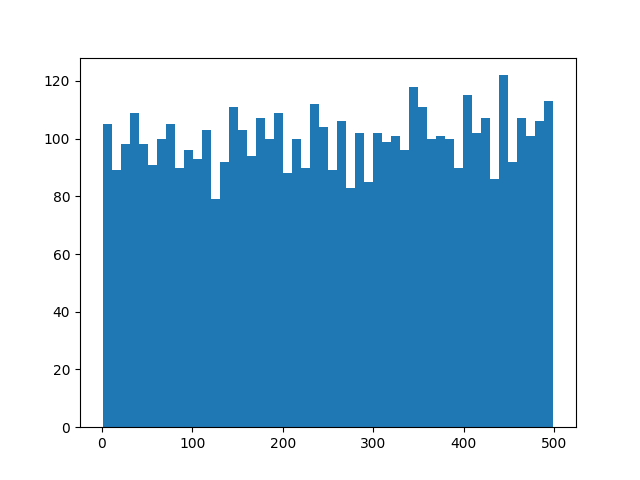
\includegraphics[width=0.3 \columnwidth]{./screenshots/Active.png}
            \caption{
                    \label{fig:Active}
                    Distribution of all Active periods.
            }
        \end{figure}
    \subsection{High Utilization}
        The creation of a High utilization workload profiles requires to have the presence of a majority of active periods rather than idle periods. Considering that we used the aforementioned method to generate active periods, we followed a similar approach in order to generate the required idle periods: by using again the \texttt{uniform(float a, float b)} method, this time centered between the minimum value $a=1\mu s$ and the maximum value $b=100 \mu s$.
        \begin{figure}[htp]
            \centering
            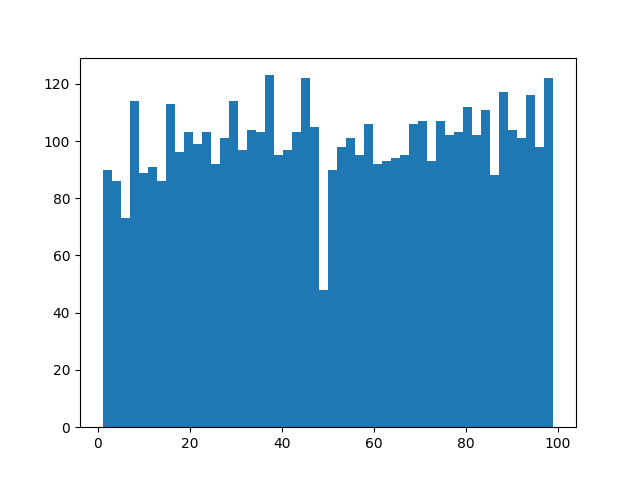
\includegraphics[width=0.3 \columnwidth]{./screenshots/Idle1.png}
            \caption{
                    \label{fig:Active}
                    Distribution of all Idle periods for the High utilization workload profile.
            }
        \end{figure}
    \subsection{Low Utilization}
        On the other hand, the creation of a Low utilization workload profile requires to generate a majority of idle periods rather than active periods. In this case, we used again the \texttt{uniform(float a, float b)} method, the minimum value $a=1\mu s$ and the maximum value $b=400 \mu s$.
        \begin{figure}[htp]
            \centering
            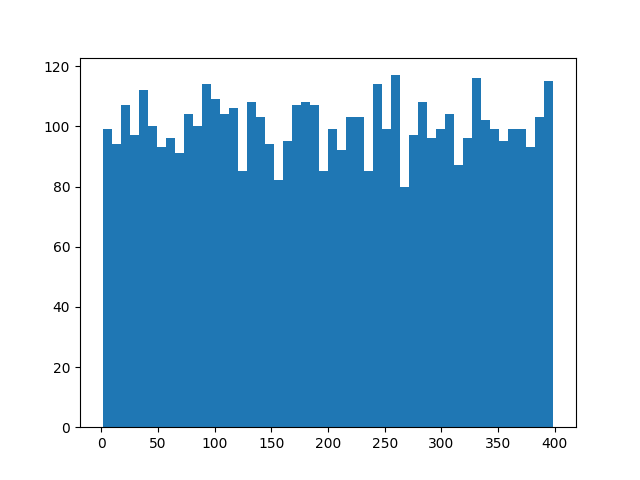
\includegraphics[width=0.3 \columnwidth]{./screenshots/Idle2.png}
            \caption{
                    \label{fig:Active}
                    Distribution of all Idle periods for the Low utilization workload profile.
            }
        \end{figure}
    \subsection{Normal distribution}
        This time, the distribution of the idle periods is required to follow a gaussian distribution, having a mean at $50 \mu s$ and a standard deviation of $20 \mu s$.
        To do that we invoked the \texttt{gauss(float mean, float std\_dev)} method of the \texttt{random} library.
        \begin{figure}[htp]
            \centering
            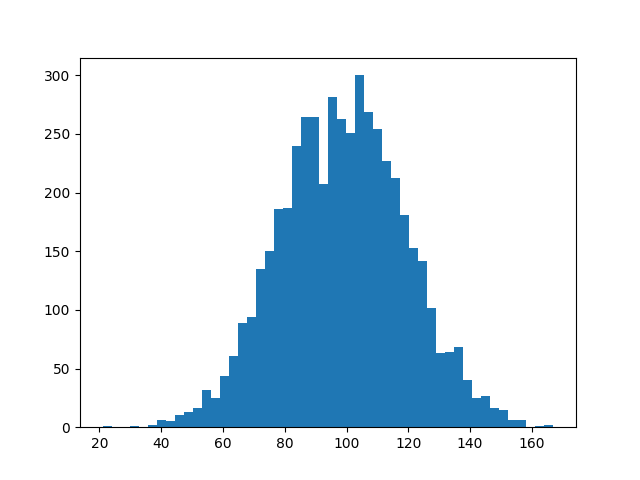
\includegraphics[width=0.3 \columnwidth]{./screenshots/Idle3.png}
            \caption{
                    \label{fig:Active}
                    Distribution of all Idle periods for the Normal distribution workload profile.
            }
        \end{figure}
    \subsection{Exponential distribution}
        This fourth distribution required to extract the idle periods following an exponential distribution, with a mean of $50 \mu s$. We used the method \texttt{expovariate(float 1/mean)}.
        \begin{figure}[htp]
            \centering
            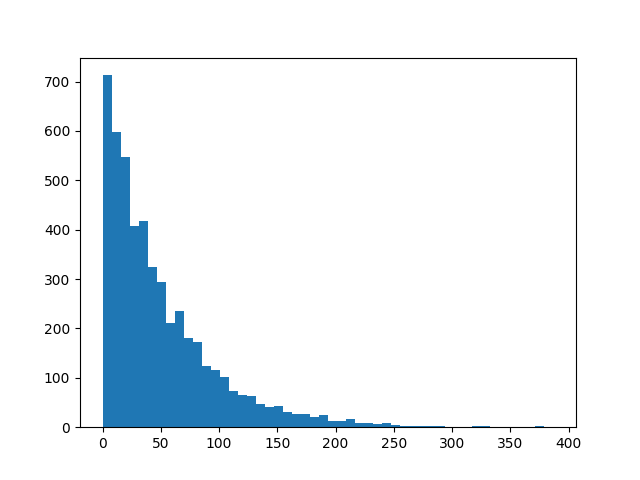
\includegraphics[width=0.3 \columnwidth]{./screenshots/Idle4.png}
            \caption{
                    \label{fig:Active}
                    Distribution of all Idle periods for the Exponential distribution workload profile.
            }
        \end{figure}
    \subsection{Tri-modal distribution}
        For this final distribution the idle values were required to be extracted from a trim-modal distribution with the following means: $50 \mu s$, $100 \mu s$, and finally $150 \mu s$. The tri-modal distribution had to be obtained using the supersposition of 3 different normal distributions with the aforementioned means and all the same standard deviation equal to $10 \mu s$.
        To generate these idle values we resorted again to the \texttt{gauss(float mean, float std\_dev)} method in order to first obtain the 3 different gaussian distributions. Finally, in order to equally extract values from them (hence obtaining the desired tri-modal behavior) we implemented a random extraction from the three normal distributions by "tossing a coin" (with three possible choices). To do that we used the \texttt{choice([0, 1, 2])} method that allowed us to select, time after time, from which gaussian we will have extracted the new idle value (each parameter in the list passed to the \texttt{choice()} method corresponds to a different gaussian  distribution).
        \begin{figure}[htp]
            \centering
            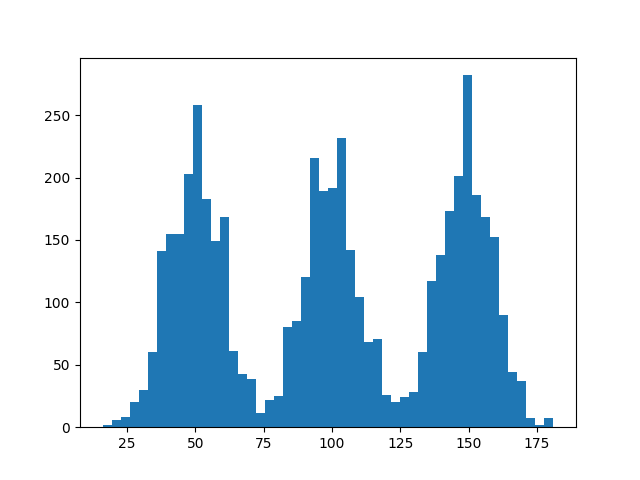
\includegraphics[width=0.3 \columnwidth]{./screenshots/Idle5.png}
            \caption{
                    \label{fig:Active}
                    Distribution of all Idle periods for the Trimodal distribution workload profile.
            }
        \end{figure}
%   _____           _     ___
%  |  __ \         | |   |__ \
%  | |__) |_ _ _ __| |_     ) |
%  |  ___/ _` | '__| __|   / /
%  | |  | (_| | |  | |_   / /_
%  |_|   \__,_|_|   \__| |____|
%
\section{Part 2: The Timeout Policy}
    \subsection{Introduction}
        For this second part of the laboratory assignment we used the workload profiles we created previously to simulate different behaviors on the provided PSM. We will discuss the results obtained dividing our work into two main cases.

        For the first case we will use a simplified version of the overall Power State Machine that can only complete transitions to and from the \texttt{Idle} state (such transitions are, of course, consequence of the use of a Dynamic Power Management technique) while, for the second case we will also finally enable the \texttt{Sleep} state of the PSM, in order to access an additional low-power state (i.e. both \texttt{Idle} and \texttt{Sleep} state will be made accessible).

        For both PSMs we will analyze the different behaviors obtained as consequences of tuning the two main parameters when considering a DPM Timeout Policy: the Timeout parameters \texttt{TtoIdle} (for both cases we will analyze) and \texttt{TtoSleep} (only for the second case).

        As we explained in the following sections, we implemented and leveraged a \texttt{python} script to launch multiple simulations while sweeping the values of the \texttt{TtoIdle} parameter, allowing us to observe the different behavior of the system assumed at each variation of the parameter.

    \subsection{Case \#1: Timeout Policy w/ \texttt{Idle} state only PSM}
        \subsubsection{The PSM}
            For this first case we use a simplified version of the overall PSM, enabling only one of the two available low-power states: the \texttt{Idle} state. A diagram of the PSM is reported in Figure(\ref{fig:PSM_case1}).

            \begin{figure}[htp]
                \centering
                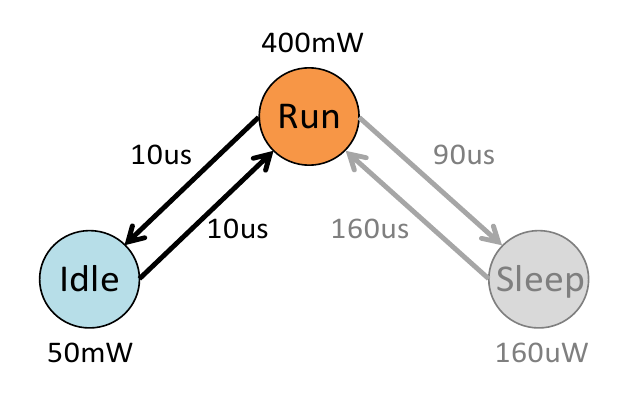
\includegraphics[width=0.4 \columnwidth]{./screenshots/PSM_case1.png}
                \caption{
                        \label{fig:PSM_case1}
                        The Power State Machine diagram used in case \#1. Only the \texttt{Idle} state has been enabled and hence reachable.
                }
            \end{figure}

            The following parameters define completely each transition of the PSM used for this first case of analysis:
            \begin{itemize}
                \item \texttt{Run} -> \texttt{Idle} transition: energy  = 10uJ, time = 10us;
                \item \texttt{Idle} -> \texttt{Run} transition: energy  = 10uJ, time = 10us;
                \item \texttt{Run} -> \texttt{Sleep} transition: energy  = 10uJ, time = 90us;
                \item \texttt{Sleep} -> \texttt{Run} transition: energy  = 30uJ, time = 160us
            \end{itemize}

            As a side note: the PSM we used includes in fact the presence of the \texttt{Sleep} state, which is however \emph{disabled} directly by the \texttt{dpm\_simulator} program that, for this first case, simply does not allow any transition to it, de facto obtaining a PSM exactly equal to the one represented in Figure(\ref{fig:PSM_case1}).

            In a Timeout policy like the one tested, the system will run in a active state when required and evaluate the necessity to reach the \texttt{Idle} state. to do that, when the workload profile cease to be active, the system waits into the \texttt{Run} state of the PSM for a certain amount of time, also called \emph{Timeout time}. In our case, the \texttt{Timeout time} refers to the \texttt{Idle} state, hence we simply called it \texttt{TtoIdle}. If the actual idle period of the workload exceeds our timeout value (considered as a threshold) then our system can transition from the \texttt{Run} state of the PSM to the \texttt{Idle} state. Of course, considering the transition delay times and non-ideal power consumptions, this timeout threshold must be carefully evaluated to not let our system consume more than if the system was simply kept operating in the \texttt{Run} state.

            By analyzing the given PSM, we can find it's \emph{Break-Even Time}. Knowing form the theory of Timeout Policies, the \emph{Break-Even Time} can be found using two formulas, depending on the intrinsic parameters of the PSM itself (non-ideal parameters):

            \begin{equation}
                Tbe = \left\{
                \begin{array}{l l}
                Ttr + Ttr \frac{Ptr - Pon}{Pon - Poff} & \quad \text{when $Ptr > Pon$}\\
                Ttr & \quad \text{when $Ptr \le Pon$}\\
                \end{array}
                \right.
            \end{equation}

            The first equation is applied in all those cases where is proven that the power required by a transition is greater than the power of the active state (in this case the \texttt{Run} state). This characteristic is intrinsic in all those systems that have a certain inertia when transitioning from a run state into a low-power one, such as rotating hard drives (or similar mechanical systems and not purely electrical).

            The second equation, on the other hand, is applied in all those cases where is proven that the power required to take a transition is lower than the power required by the active state. This is in general a characteristic of the majority of all those systems that do not include mechanical parts to be controlled.

            In our case, to firstly understand what is the formula we must apply we must compute the Power required in order to transition from the \texttt{Run} state to the \texttt{Idle} one and viceversa.

            \begin{equation}
                Ttr_{idle} = Ttr_{(Run->Idle)} + Ttr_{(Idle->Run)} = 10 \mu S + 10 \mu S = 20 \mu S
            \end{equation}
            \begin{equation}
                Ptr = \frac{Etr}{Ttr} = \frac{Etr_{(Run->Idle)} + Etr_{(Idle->Run)}}{Ttr_{(Run->Idle)} + Ttr_{(Idle->Run)}} = \frac{20 \mu j}{20 \mu s} = 1W
            \end{equation}

            Considering that $Pon = PRun = 400mW$ and $Poff = Pidle = 50 mW$ then $Ptr > Pon$, hence the first formula for the \emph{Break-Even Time} is used:

            \begin{equation}
                Tbe = Ttr + Ttr \frac{Ptr - Pon}{Pon - Poff} = 20 \mu s + 20 \mu s \frac{1W - 0.4W}{0.4W - 0.05W} = 54.3 \mu s = Tbe
            \end{equation}

            The \emph{Break-Even time} tells us that every idle time above this threshold is worth considering to transition from the \texttt{Run} state to the \texttt{Idle} one, as it allows to effectively reduce the power consumption of the entire system (considering also the non-ideal parameters like the time and energy required to complete the transitions). Again, we know from theory that having a $Tto = Tbe$ allows to have a worst-case energy consumption that is twice as higher as compared to an ideal oracle policy.

            In the following section we present the \texttt{python} script used to automatically test the behavior of the system with different values of the Timeout parameter. In general, we expect that predictions become safer (i.e. less performance penalty), but less efficient in terms of power consumption, as we increase the Timeout value. Also, at the same time, we expect that increasing the timeout value increases the wasted power (since more occasions of reaching a low power state and effectively reduce the overall power consumption are discarded).

        \subsubsection{Sweeping the Timout parameter - \texttt{Python} Script}
            To automatically complete more simulations as possible, the \texttt{python} script \texttt{simLauncher.py} has been created. The script is able to launch multiple iterations of the \texttt{dpm\_simulator} program, managing automatically the different parameters to be passed to the program and gathering all the results obtained on the power consumption, with the final goal of completing a final summary of the system's behavior (represented by a bar graph).

            The script receives as parameters the workload profile we want to test (a number going from 1 to 5), the minimum step used for the timeout sweeping and finally the maximum value the sweep can assume. Then the script, given the maximum number allowed for the sweep and the minimum sweep step, computes the total number of iterations for the simulator (each iteration corresponds to a different sweep step). Each simulation is launched by invoking the simulator feeded with the correct parameters, using the \texttt{subprocess} module.
            At each iteration the output coming from the simulator is redirected to a specific file.
            After the last iteration, all the results are then read from the corresponding output files and parsed using a regex to extract only the data referring to the final power consumption percentage gain.

            Finally, all the parsed values are inserted into a list and plotted into a bar graph, which is finally printed out as the final result coming from the \texttt{python} script.

        \subsubsection{Workload profile \#1 - High Utilization}
            For this very first workload profile we informed our \texttt{python} script to sweep from a minimum value of the timeout parameter starting from $0 \mu s$ and up to $100 \mu s$, with a minimum sweep step of $5 \mu s$. The overall results obtained are reported in Figure (\ref{fig:Idle_case1}).

            \begin{figure}[htp]
                \centering
                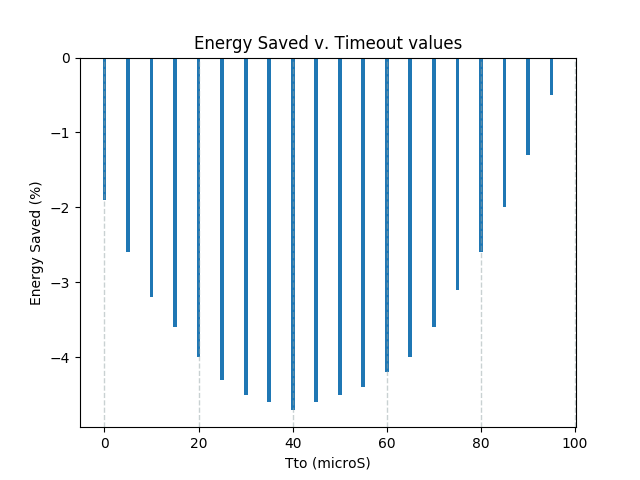
\includegraphics[width=0.6 \columnwidth]{./screenshots/Idle_case1.png}
                \caption{
                        \label{fig:Idle_case1}
                        The overall power consumption improvements we obtained with the first workload (the High Utilization one).
                }
            \end{figure}

            The following data represents the characteristics of the workload profile generated as analyzed by the simulator program:
            \begin{itemize}
                \item Total time = 1.521543s;
                \item Active time in profile = 1.266538s;
                \item Idle time in profile = 0.255005s;
            \end{itemize}

            From this data, we can evince that the overall active time is approximately 5 times longer than the overall idle time, confirming that this is a workload profile with high utilization.

            The following data, on the other hand, is tied to a single iteration/simulation: the one with timeout sweep test @ $10 \mu s$:
            \begin{itemize}
                \item Timeout waiting time = 0.052569s;
                \item Total time in state Run = 1.319107s;
                \item Total time in state Idle = 0.202436s;
                \item Total time in state Sleep = 0.000000s;
            \end{itemize}

            The first line represents the additional time spent into an active state (the \texttt{Run} state, according to our PSM) in order to observe the incoming idle period, waiting to exceed (or not) the timeout threshold of $10 \mu s$. If we do the computation, we can easily prove that \texttt{Active\_time\_in\_profile} + \texttt{Timeout\_waiting\_time} = \texttt{Total\_time\_in\_state\_run}.

            From what can be observed by looking at Figure (\ref{fig:Idle_case1}), the presence of the \texttt{Idle} state is no beneficial at all for this very first workload profile, since the overall power consumption increases in all the cases tested.

            As an example, the worst case obtained, the one with the timeout parameter set to $40 \mu s$, results into an overall power consumption increased by the $4.7\%$.
            This can be easily explained by remembering the behavior of the timeout policy: a timeout parameter equal to $40 \mu s$ implies that the system, when the workload stops to be active and enters an idle period, is kept into the active state for 40 additional $\mu s$, hence keeping consuming energy at the highest rate possible. In other words, if we consider the entire set of extracted idle periods, having a timeout parameter equal to $40 \mu s$ implies that the subset containing all the periods which duration is smaller than $40 \mu s$ is discarded a priori, hence leaving only the remaining subset in which the idle periods are greater than $40 \mu s$.

            Then, if the idle period is effectively greater than the timeout threshold the system enters the \texttt{Idle} state for the remaining time which is, in the best case scenario, equivalent to $100 \mu s - 40 \mu s = 60 \mu s$ (this implies that the overall length of the actual idle period is the greatest possible @ $100 \mu s$, considering this High Utilization workload profile).
            If we try now to observe all the other cases except the best case scenario, it is of course possible (and overall more probable) to have an overall idle period which is inferior to the maximum possible value of $100 \mu s$. Hence, the "\emph{useful}" remaining portion of the overall idle period (was equivalent to $60 \mu s$ in the best case scenario) will be of course even smaller.
            If we now remember the definition we gave previously of the \emph{Break-Even time} parameter, we see that this remaining portion of useful time can be really close to the value of the \emph{Break-Even time} we obtained previously ($54.3 \mu s$). Sometimes, if we do not consider idle time periods close to the best case scenario value ($100 \mu s$), we can obtain portions of "\emph{useful}" time that are below the \emph{Break-Even time} threshold, hence not beneficial considering the power consumption (i.e. taking the transition to the \texttt{Sleep} state will only result into an increased power consumption).

            These considerations helped us understanding why the first part of the graph (\ref{fig:Idle_case1}) curve (from $0 \mu s$ to $40 \mu s$) increases in terms of power consumption. But what about the remaining section from $40 \mu s$ to $100 \mu s$?
            The decrease in terms of power consumption, in this case, can be explained by considering that an increase of the timeout parameter effectively reduces the remaining "\emph{useful}" portion of the overall idle period (as said before) but also reduces the possibilities of having an overall idle period greater than this threshold. Hence, the decrease in power consumption is due to the fact that simply we have a decreasing number of opportunities to transition into the \texttt{Idle} state of the PSM.

        \subsubsection{Workload profile \#2 - Low Utilization}
            Following the same procedure applied before, we completed a new batch of simulations with the second workload profile. This time the idle periods are extracted from a uniform distribution and can assume values that spread from $1 \mu s$ to $400 \mu s$.
            In the following picture (\ref{fig:Idle_case2}) we can observe the overall behavior of the system when feeded with this workload.

            \begin{figure}[htp]
                \centering
                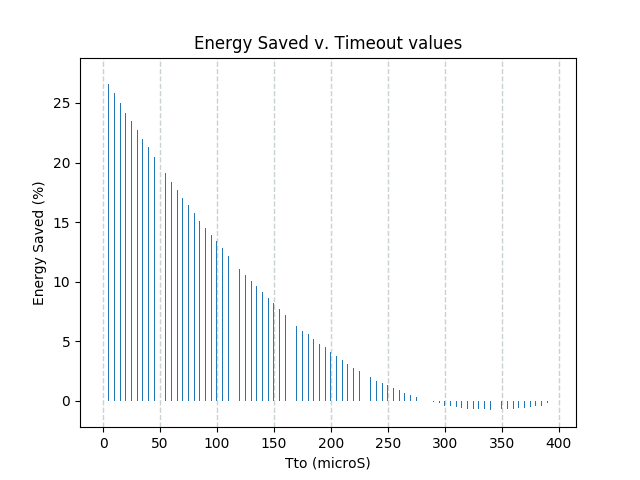
\includegraphics[width=0.6 \columnwidth]{./screenshots/Idle_case2.png}
                \caption{
                        \label{fig:Idle_case2}
                        The overall power consumption improvements we obtained with the second workload (the Low Utilization one).
                }
            \end{figure}

            The data obtained by the analysis of the workload done by the simulator is the following:
            \begin{itemize}
                \item Total time = 2.263667s;
                \item Active time in profile = 1.263454s;
                \item Idle time in profile = 1.000213s;
            \end{itemize}

            This time, the data obtained clearly demonstrates that our workload profile has an overall active time that is quite similar to the overall idle time, proving that this is a low utilization profile. Also, by looking at the graph (\ref{fig:Idle_case2}), it is clear that the timeout policy brings good energy savings, especially with lower timeout thresholds.
            The difference with the previous workload is clear if we think at the different workload profile structure: having a distribution of idle periods that is 4 times larger than the previous one allows to the system to have enough time to enter the \texttt{Idle} state and to effectively benefit from entering it. This also explains why lower timeout values bring higher benefits in terms of power consumption: less time is wasted in the \texttt{Run} state to just observe the workload and decide what to do. A small timeout time minimizes the chances of spending time at a higher consumption rate and maximizes the chances of having the system idling in a a low power state.
            While the previous case demonstrated the obvious presence of two different and opposed forces in the system, here the second contribution (the one that reduces the effectiveness of the low power state if the timeout parameter steadily increases) has the majority of the impact on the system.
            In fact, if we observe closely the graph (\ref{fig:Idle_case2}) when the timeout parameter is approximately equal to $285 \mu s$ we can see that the power consumption becomes greater if the DPM is enabled.
            At $340 \mu s$ the system reaches its higher power consumption possible. We can take a similar approach to what we have done before and analyze this behavior: when the timeout parameter is equal to $335-340 /mu s$ the remaining portion of "\emph{useful}" time is equal to $60 \mu s$, in the best case scenario (i.e. assuming we are in the longest possible idle period $400 \mu s$). If we then consider all other timeout values before the best case scenario then we can see that there's a good probability that the remaining time in which the system can stay in the \texttt{Idle} state is lower than the \emph{Break-Even time}. Hence the power consumption of the system will be higher than the same system without DPM.

        \subsubsection{Workload profile \#3 - Normal Distribution of Idle times}
            In figure (\ref{fig:Idle_case3}) we reported the behavior observed by running a batch of simulations for the third workload profile.

            \begin{figure}[htp]
                \centering
                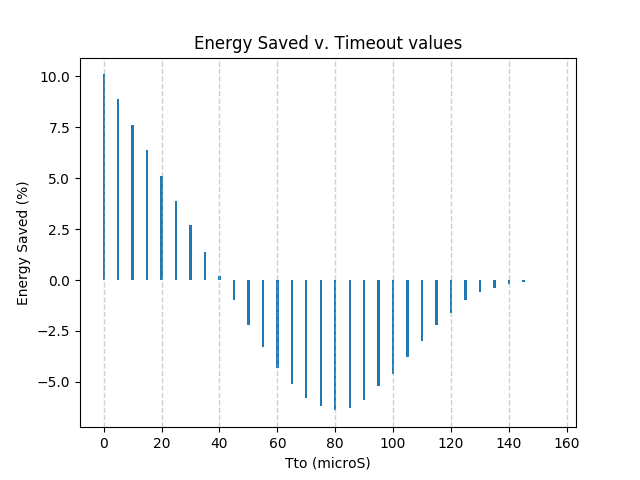
\includegraphics[width=0.6 \columnwidth]{./screenshots/Idle_case3.png}
                \caption{
                        \label{fig:Idle_case3}
                        The overall power consumption improvements we obtained with the third workload (Normal distribution of idle times).
                }
            \end{figure}

            The data obtained by the analysis of the workload done by the simulator is the following:
            \begin{itemize}
                \item Total time = 1.765396s;
                \item Active time in profile = 1.271131s;
                \item Idle time in profile = 0.494265s;
            \end{itemize}

        \subsubsection{Workload profile \#4 - Exponential Distribution of Idle times}
            In figure (\ref{fig:Idle_case4}) we reported the behavior observed by running a batch of simulations for the fourth workload profile.

            \begin{figure}[htp]
                \centering
                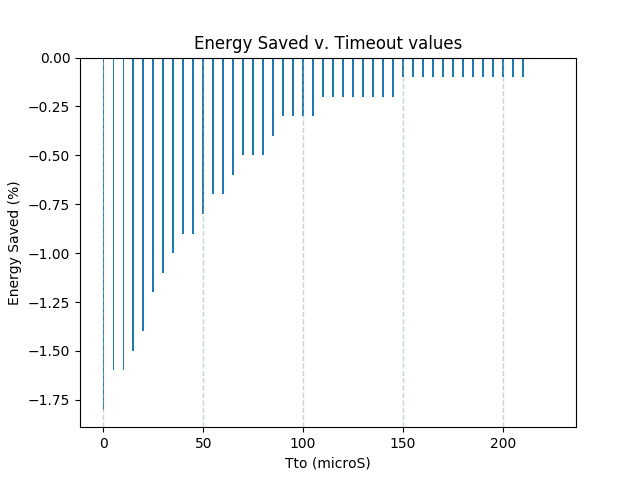
\includegraphics[width=0.6 \columnwidth]{./screenshots/Idle_case4.png}
                \caption{
                        \label{fig:Idle_case4}
                        The overall power consumption improvements we obtained with the fourth workload (Exponential distribution of idle times).
                }
            \end{figure}

            The data obtained by the analysis of the workload done by the simulator is the following:
            \begin{itemize}
                \item Total time = 1.495377s;
                \item Active time in profile = 1.245463s;
                \item Idle time in profile = 0.249914s;
            \end{itemize}

            Similarly to what we already saw with profile \#1 (the High Utilization one), here the idle periods are too short to prove a beneficial improvement on the power consumption. In fact, using DPM is, also in this case, counterproductive since the power consumption increases.

        \subsubsection{Workload profile \#5 - Tri-modal Distribution of Idle times}
            In figure (\ref{fig:Idle_case5}) we reported the behavior observed by running a batch of simulations for the fifth workload profile.

            \begin{figure}[htp]
                \centering
                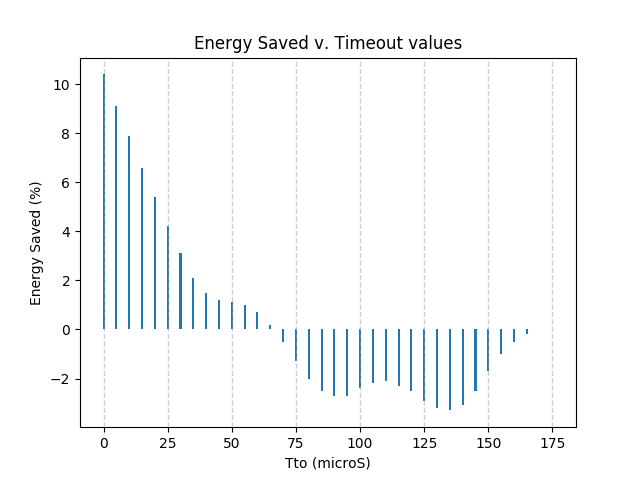
\includegraphics[width=0.6 \columnwidth]{./screenshots/Idle_case5.png}
                \caption{
                        \label{fig:Idle_case5}
                        The overall power consumption improvements we obtained with the fifth workload (Tri-Modal distribution of idle times).
                }
            \end{figure}

            The data obtained by the analysis of the workload done by the simulator is the following:
            \begin{itemize}
                \item Total time = 1.749215s;
                \item Active time in profile = 1.250748s;
                \item Idle time in profile = 0.498467s;
            \end{itemize}

    \subsection{Case \#2: Timeout Policy w/ \texttt{Idle} + \texttt{Sleep} states PSM}
        \subsubsection{The PSM}
            For this second case we must enable the second low-power state (the \texttt{Sleep} state) fo the PSM. A diagram of the original PSM is reported in Figure(\ref{fig:PSM_case2}).
            Also, the diagram of the PSM actually used is reported in Figure(\ref{fig:PSM_case3}).

            \begin{figure}[htp]
                \centering
                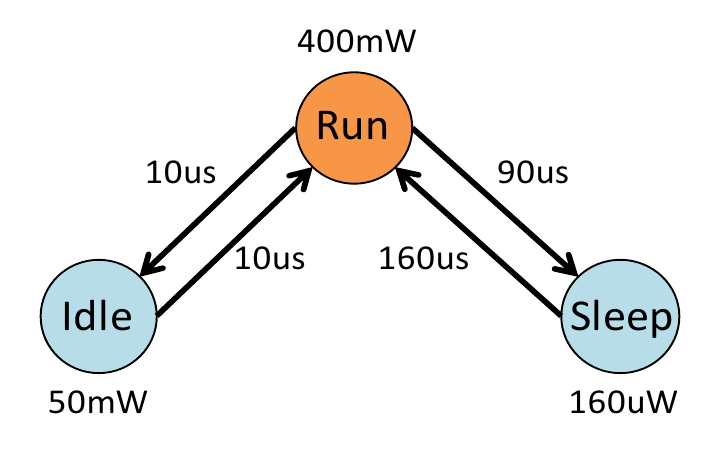
\includegraphics[width=0.35 \columnwidth]{./screenshots/PSM_case2.png}
                \caption{
                        \label{fig:PSM_case2}
                        The Power State Machine provided. Both low power states are enabled and reachable. This diagram does not actually represents the transitions implemented for our tests.
                }
            \end{figure}

            \begin{figure}[htp]
                \centering
                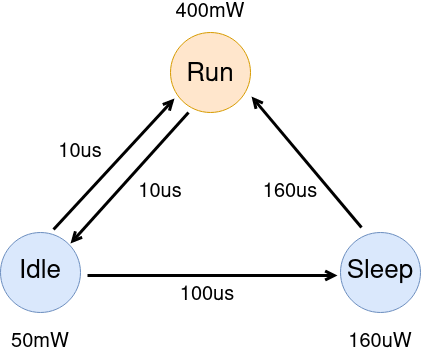
\includegraphics[width=0.35 \columnwidth]{./screenshots/PSM_case3.png}
                \caption{
                        \label{fig:PSM_case3}
                        The Power State Machine actually implemented. Both low power states are enabled and reachable. Notice the additional transition form \texttt{Idle} to \texttt{Sleep} and the removed transitions with respect to the PSM diagram provided.
                }
            \end{figure}


            The following parameters define completely each transition of the PSM used for this second case of analysis:
            \begin{itemize}
                \item \texttt{Run} -> \texttt{Idle} transition: energy  = 10uJ, time = 10us;
                \item \texttt{Idle} -> \texttt{Run} transition: energy  = 10uJ, time = 10us;
                \item \texttt{Idle} -> \texttt{Sleep} transition: energy  = 20uJ, time = 100us;
                \item \texttt{Sleep} -> \texttt{Run} transition: energy  = 30uJ, time = 160us
            \end{itemize}

            The PSM we used in order to test the new configuration that includes the \texttt{Sleep} state is visible in the second diagram (\ref{fig:PSM_case3}).
            The behavior is defined as follows: if the workload profile enters an idle period then both the timeout timers are activated (\texttt{Idle} and \texttt{Sleep} timeouts). Assuming the \texttt{Sleep} timeout threshold is greater than the \texttt{Idle} timeout threshold, if the \texttt{Idle} timeout timer expires and the workload is still in an idle state, then the system takes the transition from the \texttt{Run} state to the \texttt{Idle} one.
            Also the second threshold is checked: if the timeout timer associated to the \texttt{Sleep} state expires, then the system can also move to the \texttt{Sleep} state. This transition is represented in the diagram by the arrow going from the \texttt{Idle} state to the \texttt{Sleep} one. Please, notice how the transition has been implemented: the transitions costs for both time and power consumption include both the costs necessary to go from \texttt{Idle} to \texttt{Run} and then from \texttt{Run} to \texttt{Sleep} state. That's why we decided to report also the provided diagram (\ref{fig:PSM_case2}), that represents the "logical" transitions, meanwhile the second diagram (\ref{fig:PSM_case3}) represents the "physical" ones.
            Finally, whenever the workload resumes from the inactive state and goes back into an active state the two transitions going from the \texttt{Idle} (or \texttt{Sleep}) states can be taken to revert the system into the \texttt{Run} state.

        \subsubsection{The modified \texttt{dpm\_simulator}}
            To add the capability to the simulator to reach the \texttt{Sleep} state, we were asked to add the code to implement the policy. The functionality is pretty simple: at each instant, we check if the current time has overcome the first timeout threshold (associated to the \texttt{Idle} state). If it is the case, the system can reach the \texttt{Idle} state. If not the system will remain into the \texttt{Run} state. Once we declared that, at least, the system is eligible to reach the \texttt{Idle} state, we check again if it can reach the \texttt{Sleep} state. To do that, we check if the current time is greater than the second timeout threshold (associated to the \texttt{Sleep} state). At the same time we also check if the second threshold is effectively greater than the first one (this control, unnecessary due to our assumption that the \texttt{Sleep} timeout is always larger than the \texttt{Idle} timeout, is however necessary considering the integration of our simulator with the \texttt{python} script as we will see in the next sections). If both the conditions reveal to be true, then the system is eligible to reach the \texttt{Sleep} state.
            As a side note: by observing the conditions imposed above one could argue that such implementation may allow a transition directly from the \texttt{Run} state to the \texttt{Sleep} one. However, such transition is impossible firstly because it has not been implemented in the PSM file feeded as input to the simulator and secondly because of the internal time-incremental logic the simulator adopts (that guarantees that the \texttt{Idle} state will be reached before the \texttt{Sleep} one).

            In the following section we briefly present the modifications we made to the original \texttt{python} script used to automatically test the behavior of the system with different values of the two Timeout parameters.

        \subsubsection{Sweeping the \texttt{Sleep} Timout parameter - \texttt{Python} Script}
            With the modifications made to the original \texttt{python} script, we are now able to launch multiple iterations of the \texttt{dpm\_simulator} program, by keeping fixed the \texttt{Idle} timeout parameter and by seeping the \texttt{Sleep} parameter on top of it. The script is again able to manage automatically the different parameters to be passed to the program and gathering all the results obtained on the power consumption, with the final goal of completing a final summary of the system's behavior (represented by a bar graph).

            For each workload profile, multiple runs of the script have been made (in the previous case just one single run of the script was necessary). This behavior is necessary in order to test the system with different conditions on the \texttt{Idle} timeout: the script, being derived from the first version we used before, is able to sweep only one timeout parameter at a time, in this case only the \texttt{Sleep} one. To "sweep" also the \texttt{Idle} timeout parameter, we decided to launch multiple times the same script by fixing at each time a different value.

            The script receives as parameters the workload profile we want to test (a number going from 1 to 5), the minimum step used for the timeout sweeping, the fixed value for the \texttt{Idle} timeout parameter and finally the maximum value the sweep of the \texttt{Sleep} timeout can assume. The script, given the maximum number allowed for the sweep and the minimum sweep step, computes then the total number of iterations for the simulator (each iteration corresponds to a different sweep step). As before, the results are saved into multiple files and finally collected to draw a graph representing the behavior of the system.

        \subsubsection{Workload profile \#1 - High Utilization}
            For this first case we launched 5 different simulations with 5 different \texttt{Idle} timeout values. For each simulation, the script sweeped the \texttt{Sleep} timeout parameter from $0 \mu s$ to $1 \mu s$. We report in Figure (\ref{fig:Sleep_case1}) just one of them: the batch of simulations done while fixing the \texttt{Idle} timeout parameter @ $40 \mu s$ (all the other batches follow the very same principle).

            \begin{figure}[htp]
                \centering
                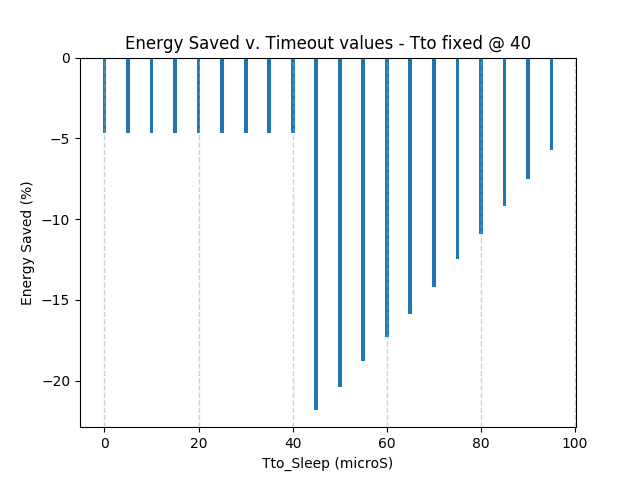
\includegraphics[width=0.6 \columnwidth]{./screenshots/Sleep_case1.png}
                \caption{
                        \label{fig:Sleep_case1}
                        The overall power consumption improvements we obtained with the first workload (the High Utilization one).
                }
            \end{figure}

            Again, like we saw with the previous tests, this workload profile doesn't benefit at all of DPM, since the extracted idle periods are too short to reduce the power consumption, considering the characteristics of the system. In this case, with the \texttt{Sleep} state enable and reachable, the results are even poorer than before.
            From the previous graph (\ref{fig:Sleep_case1}) we can observe that the power consumption remains stable @ $-4.7\%$: this value shows exactly the behavior of the system as if only the \texttt{Idle} state was reachable (in fact, the \texttt{Sleep} state becomes reachable only if its related timeout threshold is exceeded, which we assumed cannot be smaller or equal the \texttt{Idle} timeout threshold).
            Only when the \texttt{Sleep} timeout parameters is set grater than the \texttt{Idle} threshold the system can reach the corresponding \texttt{Sleep} state. In our graph, this behavior is clearly visible starting from the simulation done @ $45 \mu s$.
            Again, like to what seen before, as we increase the timeout threshold the power consumption penalty decreases since less and less idle periods can actually be taken by the machine.

        \subsubsection{Workload profile \#2 - Low Utilization}
        Like in the previous case, we report in Figure (\ref{fig:Sleep_case2}) just one batch of simulations: the \texttt{Idle} timeout parameter has been fixed @ $150 \mu s$ (all the other batches follow the very same principle).

        \begin{figure}[htp]
            \centering
            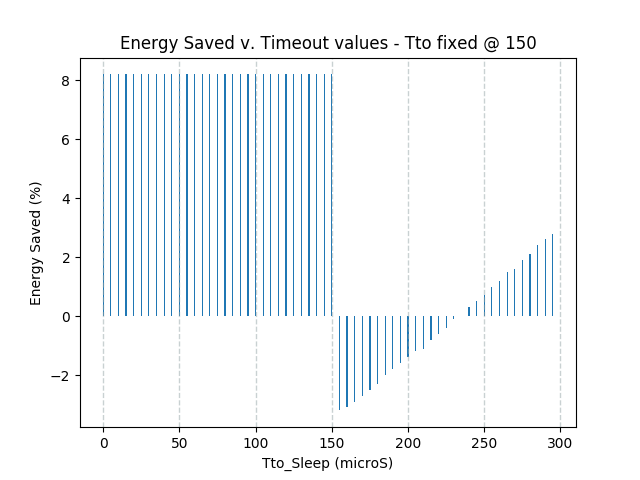
\includegraphics[width=0.6 \columnwidth]{./screenshots/Sleep_case2.png}
            \caption{
                    \label{fig:Sleep_case2}
                    The overall power consumption improvements we obtained with the second workload (the Low Utilization one).
            }
        \end{figure}

        \subsubsection{Workload profile \#3 - Normal distribution of Idle periods}
        \begin{figure}[htp]
            \centering
            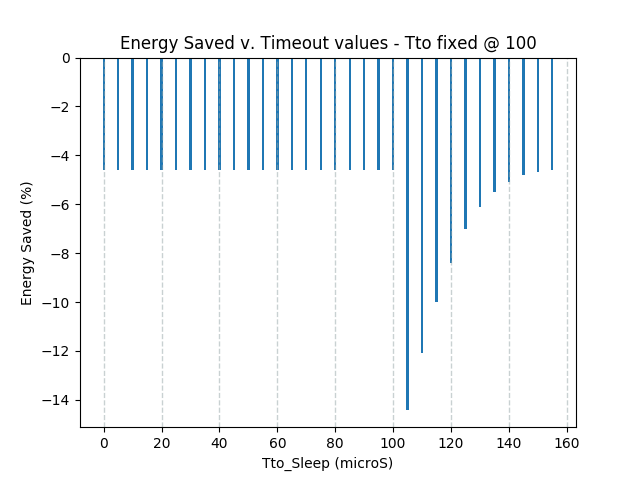
\includegraphics[width=0.6 \columnwidth]{./screenshots/Sleep_case3.png}
            \caption{
                    \label{fig:Sleep_case3}
                    The overall power consumption improvements we obtained with the third workload (Normal distribution of ilde times).
            }
        \end{figure}

        \subsubsection{Workload profile \#4 - Exponential distribution of Idle periods}
        \begin{figure}[htp]
            \centering
            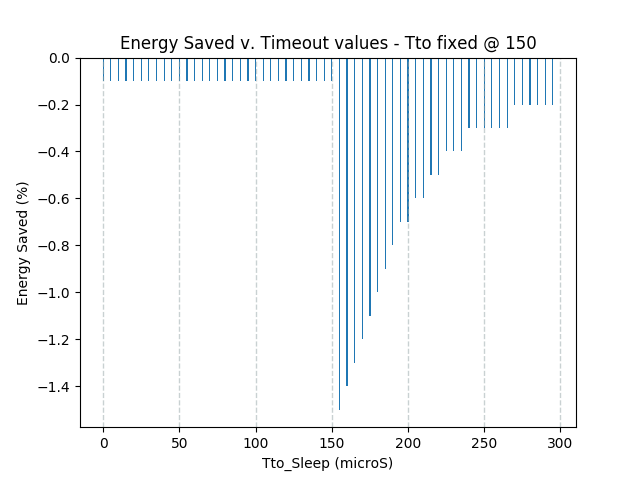
\includegraphics[width=0.6 \columnwidth]{./screenshots/Sleep_case4.png}
            \caption{
                    \label{fig:Sleep_case4}
                    The overall power consumption improvements we obtained with the fourth workload (Exponential distribution of ilde times).
            }
        \end{figure}

        \subsubsection{Workload profile \#5 - Tri-Modal distribution of Idle periods}
        \begin{figure}[htp]
            \centering
            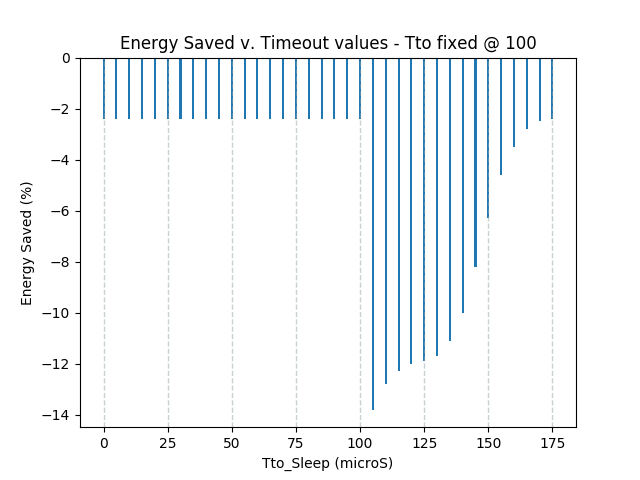
\includegraphics[width=0.6 \columnwidth]{./screenshots/Sleep_case5.png}
            \caption{
                    \label{fig:Sleep_case5}
                    The overall power consumption improvements we obtained with the fifth workload (Tri-Modal distribution of ilde times).
            }
        \end{figure}

%   _____           _     ____
%  |  __ \         | |   |___ \
%  | |__) |_ _ _ __| |_    __) |
%  |  ___/ _` | '__| __|  |__ <
%  | |  | (_| | |  | |_   ___) |
%  |_|   \__,_|_|   \__| |____/
%
%
\section{Part 2: The History Policy}
    \subsection{Introduction}
        For this second part of the laboratory assignment we used the workload profiles we created previously to simulate different behaviors on the provided PSM. We will discuss the results obtained dividing our work into two main cases.

        For the first case we will use a simplified version of the overall Power State Machine that can only complete transitions to and from the \texttt{Idle} state (such transitions are, of course, consequence of the use of a Dynamic Power Management technique) while, for the second case we will also finally enable the \texttt{Sleep} state of the PSM, in order to access an additional low-power state (i.e. both \texttt{Idle} and \texttt{Sleep} state will be made accessible).

        For both PSMs we will analyze the different behaviors obtained as consequences of tuning the two main parameters when considering a DPM Timeout Policy: the Timeout parameters \texttt{TtoIdle} (for both cases we will analyze) and \texttt{TtoSleep} (only for the second case).

        As we explained in the following sections, we implemented and leveraged a \texttt{python} script to launch multiple simulations while sweeping the values of the \texttt{TtoIdle} parameter, allowing us to observe the different behavior of the system assumed at each variation of the parameter.

    \subsection{Case \#1: Timeout Policy w/ \texttt{Idle} state only PSM}
        \subsubsection{The PSM}


        \subsection{PWM wave generation}
        The PWM generation is done by leveraging the Flex Timer 0 embedded into the microprocessor. Once the timer initialized, a PWM wave is created following the given parameters, such as the frequency and the duty cycle. Finally the wave is feeded to the pin mapped to the embedded RGB LED on the NXP board.

        \begin{itemize}
            \item \texttt{BSP\_FTM0\_PWM\_Init()}: This is the initialization function for the timer: the clock is enabled for port D and each pin of the RGB LED is set as a function of the relative FlexTimer0 channel (the RED one is associated to channel \#0, the GREEN one is associated to channel \#1 and the BLUE one to channel \#2).
            \item \texttt{BSP\_FTM0\_PWM\_set(CPU\_INT32U PWMfrequency, CPU\_INT08U dutyCycle)}: This function, given the two parameters, computes the value for the \texttt{modulo} register and sets an initial value for the hardware counter of the timer. The \texttt{modulo} value is simply computed by dividing the clock frequency of the timer ($80MHz$ in our case) by the wanted PWM frequency. In our case, given the $10KHz$ PWM frequency given by the requirements, the final value will be 8000. It is useful to underline the importance of this value because the \texttt{FTM0->MOD} register can accept values up to 65535 (16-bit register). If a lower value of the PWM frequency is needed we could probably compute a value for the \texttt{modulo} register that cannot be represented on 16 bits: in this case the use of the prescaler is mandatory. Since the PWM frequency value adopted in our program is fixed and below the threshold, no logic has been implemented to automatically adjust the prescaler consequently to the value of the \texttt{PWMfrequency} parameter. Finally, the function calls the \texttt{setDutyCycle(BSP\_LED ledColor, CPU\_INT32U modulo, CPU\_INT08U dutyCycle)} static function.
            \item \texttt{setDutyCycle(BSP\_LED ledColor, CPU\_INT32U modulo, CPU\_INT08U dutyCycle)}: this function is defined as \texttt{static} and so its visibility is limited only to \texttt{bsp\_timer.c} source file. This function, given the \texttt{dutyCycle} parameter and the previously computed \texttt{modulo} parameter, sets the according value for register \texttt{FTM0->CONTROLS[i].CnV} (where i = 0, 1, 2 and corresponds to the number of the channel of which we modify the value of the PWM). Finally the \texttt{BSP\_FTM0\_PWM\_EnableLED(BSP\_LED ledColor)} function is called, which will finally enable the wanted timer channel, accordingly to the requested color of the LED.
            \item \texttt{BSP\_FTM0\_PWM\_EnableLED(BSP\_LED ledColor)}: this function, given the requested LED color, enables the corresponding timer channel.
            \item \texttt{BSP\_FTM0\_PWM\_ChangeDutyCycle(BSP\_LED ledColor, CPU\_INT32U PWMfrequency, CPU\_INT08U dutyCycle)}: This function is used to expose and to wrap the \texttt{setDutyCycle(BSP\_LED ledColor, CPU\_INT32U modulo, CPU\_INT08U dutyCycle)} static function to the external software modules. This function will be used into the pushbutton interrupt service routine.
        \end{itemize}

        \subsection{LED color switching}
        During the execution of the \texttt{AcquireADCTask} infinite loop, an interrupt is raised if the pushbutton is pressed by the user: this will cause the LED color to change following the requested sequence.
        Initially the idea was to create two separate tasks where the second one could manage the pushbutton status by acting in a polling fashion: after the execution of the first task (which would have had a higher priority) the second task would have been launched (a synchronization semaphore would be needed) that would have checked the pushbutton status acting consequently of its pressure. However, this solution would have added intrinsic latency due to both the alternation of the two tasks (context switch) and the polling approach (for instance, what would happen if the pushbutton is pressed just after the \texttt{read\_status} statement? We would need to wait the completion of the new instance of task \#1, waiting to gain access again to task \#2).

        Using an interrupt approach, on the contrary, eliminates the latency of the polling approach and the complications due to the dual task handling.
        Let's now investigate the functions associated to the pushbutton, along with the Interrupt Service Routine:

        \begin{itemize}
            \item \texttt{BSP\_Switch\_Init()}: This function initializes the two pushbutton embedded on the board: \emph{Switch3} and \emph{Switch2}. For this assignment only \emph{Switch2} will be used, however I decided to include the configuration of \emph{Switch3} for future usecases. This function enables the clock to Port C, sets as input both switches pins and enables \emph{Switch2} to raise an interrupt only by reacting to a falling edge transition. Finally it declares the usage of the Interrupt Handler associated to \emph{Switch2}.
            \item \texttt{SW2\_int\_hdlr(void)}: This is the Interrupt Handler associated to \emph{Switch2}. If this pushbutton is pressed, an interrupt is raised and the processor will start serving this part of the code. The status of the switch is read using the function \texttt{BSP\_Switch\_Read (BSP\_SWITCH sw)}: if the pushbutton has been pressed then the LED color is changed accordingly to the current color and the requested color sequence, using the function \texttt{BSP\_FTM0\_PWM\_ChangeDutyCycle(BSP\_LED ledColor, CPU\_INT32U PWMfrequency, CPU\_INT08U dutyCycle)}.
            \item \texttt{BSP\_Switch\_Read (BSP\_SWITCH sw)}: this function reads the input data register of the selected pushbutton.
        \end{itemize}

        Other functions like the ones that can be found in \texttt{bsp\_led.c} will not be discussed since after a proper code cleanup they became unused: I decided to leave the entire \texttt{bsp\_led.c} and the functions like \texttt{BSP\_LED\_Init (void)}, \texttt{BSP\_LED\_On (BSP\_LED color)}, \texttt{BSP\_LED\_Off (BSP\_LED color)} and \texttt{BSP\_LED\_Toggle (BSP\_LED color)} for next use cases that another user may want to implement.

        \newpage

        \subsection{Flow Diagram for \texttt{AcquireADCTask}}



    \end{document}